\documentclass[]{osa-article}

%% Select the journal you're submitting to
%% oe, boe, ome, osac, osajournal
\journal{osajournal}
% Key:
% Express journals must have the correct journal selected:
% {oe} Optics Express
% {boe} Biomedical Optics Express
% {ome} Optical Material Express
% {osac} OSAC Continuum
% Other OSA journals may use:
% {osajournal} Applied Optics, Advances in Optics and Photonics, Journal of the Optical Society of America A/B, Optics Letters, Optica, Photonics Research

% Uncomment if submitting to Photonics Research.
% ONLY APPLICABLE FOR \journal{osajournal}
% \setprjcopyright

% Set the article type
\articletype{Research Article}
% Note that article type is not required for Express journals (OE, BOE, OME and OSAC)

% Talon's custom libraries
\usepackage{empheq}
% \usepackage{bm}

% Talon's custom commands
\DeclareMathAlphabet{\mathcal}{OMS}{cmsy}{m}{n}
\newcommand{\tensor}[1]{\overset{\text{\tiny$\leftrightarrow$}}{\mb{#1}}}
\newcommand{\argmin}{\arg\!\min}
\newcommand{\me}{\mathrm{e}}
\providecommand{\e}[1]{\ensuremath{\times 10^{#1}}} 
\providecommand{\mb}[1]{\mathbf{#1}}
\providecommand{\msf}[1]{\mathsf{#1}}
\providecommand{\mf}[1]{\mathfrak{#1}}
\providecommand{\mc}[1]{\mathcal{#1}}
\providecommand{\ro}{\mathbf{\mathbf{r}}_o}
\providecommand{\so}{\mathbf{\hat{s}}_o}
\providecommand{\rb}{\mathbf{r}_b}
\providecommand{\rbm}[1]{r_b^{\text{m}}}
\providecommand{\rd}{\mathbf{r}_d}
\providecommand{\rdf}{\mathpzc{r}_d}
\providecommand{\mh}[1]{\mathbf{\hat{#1}}}
\providecommand{\mbb}[1]{\mathbb{#1}}
\providecommand{\bs}[1]{\boldsymbol{#1}}
\providecommand{\bv}{\bs{\nu}}
\providecommand{\bsh}[1]{\hat{\boldsymbol{#1}}}
\providecommand{\nan}{\left(\frac{\text{NA}}{n_o}\right)}
\providecommand{\lmsum}{\sum_{\ell=0}^\infty\sum_{m=-\ell}^{\ell}}
\providecommand{\intr}[1]{\int_{\mbb{R}^{#1}}}
\providecommand{\ints}[1]{\int_{\mbb{S}^{#1}}}
\providecommand{\tb}[1]{\textcolor{blue}{#1}}
\DeclareFontFamily{OT1}{pzc}{}
\DeclareFontShape{OT1}{pzc}{m}{it}{<-> s * [1.10] pzcmi7t}{}
\DeclareMathAlphabet{\mathpzc}{OT1}{pzc}{m}{it}
\newcommand{\eqname}[1]{\tag*{#1}}
\newcommand*\widefbox[1]{\fbox{\hspace{1em}#1\hspace{1em}}}

\begin{document}

\title{Spatio-angular fluorescence microscopy I. Basic theory}

\author{Talon Chandler,\authormark{1,*} Author order TBD,\authormark{2,*} and Patrick La Rivi\`ere \authormark{1}}

\address{\authormark{1}University of Chicago, Department of Radiology, Chicago, Illinois 60637, USA\\
\authormark{2}Publications Department, The Optical Society, 2010 Massachusetts Avenue NW, Washington, DC 20036, USA\\
\authormark{3}Currently with the Department of Electronic Journals, The Optical Society, 2010 Massachusetts Avenue NW, Washington, DC 20036, USA}

\email{\authormark{*}talonchandler@talonchandler.com} %% email address is required

%\homepage{talonchandler@talonchandler.com} %% author's URL, if desired

%%%%%%%%%%%%%%%%%%% abstract %%%%%%%%%%%%%%%%
%% [use \begin{abstract*}...\end{abstract*} if exempt from copyright]

\begin{abstract*}
  We introduce the basic elements of a spatio-angular theory of fluorescence
  microscopy. We start by modeling a microscope imaging an ensemble of in-focus
  fluorescent dipoles as a linear Hilbert-space operator with domain
  $\mbb{L}_2(\mbb{R}^2\times\mbb{S}^2)$ and range $\mbb{L}_2(\mbb{R}^2)$, and we
  express the operator in terms of four different sets of object-space basis
  functions. We show that the operator takes a particularly convenient form when
  expressed in a basis of spatial and spherical harmonics---a form we call the
  spatio-angular transfer function (SATF). We demonstrate our formalism by
  analyzing a single-view paraxial epi-fluorescence microscope without using the
  monopole or scalar approximations. We show that this microscope has an angular
  band limit, and we demonstrate the value of the transfer function approach by
  efficiently simulating the imaging process with simple phantoms. Notably, we
  show that information about the out-of-plane orientation of ensembles of
  in-focus fluorophores is recorded by paraxial epi-fluorescence microscopes. We
  discuss the implications of our analysis for all quantitative fluorescence
  microscopy studies and lay out a path towards a complete theory.
\end{abstract*}

\section{Introduction}

Fluorescence microscopes are widely used in the biological sciences for
measuring the spatial distribution of fluorophores throughout a sample [cite].
While an unprocessed fluorescence micrograph reports the approximate
distribution of fluorophores throughout a sample, all microscopes are
diffraction limited [cite], so the image is a blurred version of the true
fluorophore distribution. 

Restoration techniques attempt to recover the true distribution of fluorophores
using the measured data and a model of the imaging process. A model of the
imaging process can be obtained theoretically (by mathematically modeling the
instrument under idealized conditions), experimentally (by measuring the
instrument's response to a known input), or by a combination of theory and
experiment (by measuring parameters of an instrument model). In all cases the
accuracy of the restored fluorophore distribution is limited by the accuracy of
the imaging model. All theoretical imaging models make simplifying
approximations that limit the accuracy of restorations, so it is important to
verify that the approximations introduce an acceptable level of error. This work
investigates the errors introduced by two common approximations in models of
fluorescence microscopes---the \textit{monopole approximation} and the
\textit{scalar approximation}.

The widely-used monopole model treats fluorophores as molecules that absorb and
emit light isotropically. Despite their use in models, monopole
absorber/emitters do not exist in nature. All real fluorophores absorb and emit
light anisotropically, and in this work we investigate the more realistic dipole
model of fluorophores. Since the absorption and emission patterns of many widely
used fluorophores including green fluroescent protein (GFP) are known to be well
described by the dipole model [cite Inoue], we start by considering the dipole
model before higher-order multipole models.

The scalar approximation is another widely-used approximation in fluorescence
microscopy. The scalar approximation models the propagation of light using a
scalar-valued field $U$ instead of the more realistic vector-valued electric
field $\mb{E}$. Although the scalar model yields realistic results in many
cases, the scalar field ignores polarization-dependent effects. The absorption
and emission response of dipoles strongly depends on the polarization of the
fields, so we need to use an electromagnetic model of light propagation to
accurately model a microscope imaging dipoles.

This work lies at the intersection of three classes of fluorescence microscopy:
(1) single molecule localization microscopy (SMLM), (2) spatial ensemble
fluorescence microscopy including widefield, confocal, and light-sheet
techniques, and (3) polarized fluorescence microscopy. We briefly review these
three classes and focus on their use of the monopole and scalar approximations.

The SMLM community has pioneered the use of rigorous electromagnetic models of
fluorescence microscopes \cite{backer2014, lieb2004} [cite Novotny]. When a
single molecule is fluorescing in the sample, the measured intensity pattern is
strongly dependent on the orientation of the emitting molecule. Backlund [cite]
and Lew [cite] \cite{backlund2014} have shown that ignoring the orientation of
fluorophores can bias position estimates, so the most accurate SMLM experiments
must jointly estimate the position and orientation of each molecule.

Meanwhile, most fluorescence microscopists image ensembles of fluorophores and
restore their images without considering the role that the monopole and scalar
approximations play in the restoration process. A typical fluorescence
microscopist is only interested in the spatial distribution of fluorophores, so
they reason that they can ignore the orientation of the emitters.

A smaller community of microscopists is interested in measuring the orientation
of ensembles of fluorophores \cite{mehta2016} [Forkey, Goldman, Moerner,
Oldenbourg]. These techniques typically use polarized illumination or polarized
detection to make multiple measurements of the same object. Current angular
restoration techniques use a model of the dipole excitation and emission
processes [Fourkas] to recover the orientation of fluorophores using pixel-wise
arithmetic, but these techniques do not perform any spatial restoration so they
do not use all of the available information. To our knowledge no work has been
done to model the complete spatio-angular response of fluorescence microscopes
to ensembles of oriented fluorophores.

We begin in Section \ref{sec:theory} by formulating the imaging problem
mathematically. We start with an abstract description of fluorescence imaging
systems and extend the usual monopole imaging model to dipoles. Along the way we
introduce transfer functions that will allow us to efficiently simplify our
analysis of spatio-angular microscopes. In Section \ref{sec:results} we use the
mathematical tools we developed in Section \ref{sec:theory} to analyze and
simulate a single-view paraxial epi-fluorescence microscope, and we demonstrate
our model with four simple phantoms. Finally, in Section \ref{sec:discussion} we
discuss the results and their broader implications.

\section{Theory}\label{sec:theory}
We begin our analysis with the abstract Hilbert space formalism of Barrett and
Myers \cite{barrett2004}. Our first task is to formulate the imaging process as
a mapping between two Hilbert spaces $\mc{H}: \mbb{U} \rightarrow \mbb{V}$, where
$\mbb{U}$ is a set than contains all possible objects, $\mbb{V}$ is a set that
contains all possible datasets, and $\mc{H}$ is a model of the instrument that
maps between these two spaces. We denote (possibly infinite-dimensional)
Hilbert-space vectors in $\mbb{U}$ with $\mb{f}$, Hilbert-space vectors in
$\mbb{V}$ with $\mb{g}$, and the mapping between the spaces with
\begin{align}
  \mb{g} = \mc{H}\mb{f}.
\end{align}

Once we have identified the spaces $\mbb{U}$ and $\mbb{V}$, we can start
expressing the mapping between the spaces in a specific object-space and
data-space basis. In most cases the easiest mapping to find uses a
delta-function basis---we expand object and data space into delta functions,
then express the mapping as an integral transform. After finding this mapping we
can start to investigate the same mapping in different bases.

The above discussion is quite abstract, but it is a powerful point of view that
will enable us to draw new conclusions about all fluorescence microscopes. In
Section \ref{sec:monopole} we will demonstrate the formalism by examining a
familiar monopole imaging model, and we will show that the point spread
function and the optical transfer function are mappings between object and data
space expressed in two different bases. In Section \ref{sec:dipole} we will
extend the monopole imaging model to dipoles and examine the mapping in four
different bases. 

\subsection{Monopole imaging in different bases}\label{sec:monopole}
We start by considering a microscope that images a field of in-focus monopoles
by recording the irradiance on a two-dimensional detector. This section treads
familiar ground, but it serves to establish the concepts and notation that will
be necessary when we extend to the dipole case.

We can represent the object as a function that assigns a real number to each
point on a plane, so we identify object space as
$\mbb{U} = \mbb{L}_2(\mbb{R}^2)$. Similarly, we have a two-dimensional detector
that measures a real number at every point on a plane, so data space is the same
set $\mbb{V} = \mbb{L}_2(\mbb{R}^2)$.

Next, we name the representations of our object and data in a specific basis. In
a delta function basis the object can be represented by a function $f(\ro)$
called the \textit{spatial monopole density}---the number of monopoles per unit
area at the two-dimensional position $\ro$. Similarly, in a delta function basis
the data can be represented by a function $g'(\rd')$ called the
\textit{irradiance}---the power received by a surface per unit area at position
$\rd'$. It may seem pedantic to emphasize that these representations are in a
delta function basis, but we highlight this point to make it clear that the
delta function basis is not special---we can choose a different basis at will.

A reasonable starting point is to assume that the relationship between the
object and the data is \textit{linear}---this is usually true in fluorescence
microscopes since fluorophores emit incoherently, so a scaled sum of
fluorophores will result in a scaled sum of the irradiance patterns created by
the individual fluorophores. If the mapping is linear, we can write the
irradiance as a weighted integral over a field of monopoles
\begin{align}
g'(\rd') = \int_{\mbb{R}^2}d\ro\, h'(\rd',\ro)f(\ro), \label{eq:fwdmono}
\end{align}
where $h'(\rd{}', \ro{})$ is the irradiance at position $\rd'$ created by a
point source at $\ro$.

The irradiance pattern measured by many fluorescence microscopes can be modeled
(at least approximately) as a magnifier with shift-invariant blur
\begin{align}
  g'(\rd') = \int_{\mbb{R}^2}d\ro\, h'(\rd' - m\ro)f(\ro), 
\end{align}
where $m$ is a magnification factor. To simplify our analysis we define a
demagnified detector coordinate $\rd = \rd'/m$ and a normalization factor that
corresponds to the total power incident on the detector plane due to a point
source $P_{\text{mono}} = \int_{\mbb{R}^2}d\mb{r}\,h'(m\mb{r})$. We use these scaling
factors to define the \textit{point spread function} as
\begin{align}
  h(\rd - \ro) = \frac{h'(m[\rd - \ro])}{P_{\text{mono}}},
\end{align}
and the \textit{scaled irradiance} as
\begin{align}
  g(\rd) = \frac{g'(m\rd)}{P_{\text{mono}}}.
\end{align}
With these definitions we can express the mapping between the object and the
data as a familiar convolution
\begin{align}
  g(\rd) = \int_{\mbb{R}^2}d\ro\, h(\rd - \ro)f(\ro),  \label{eq:lsi}
\end{align}
which will allow us to analyze this class of microscopes without carrying
magnification or normalization factors. We will mostly be using scaled
coordinates, so we have adopted a slightly unusual convention of using primes to
denote unscaled coordinates.

We have chosen to normalize the point spread function so that
\begin{align}
  \int_{\mbb{R}^2}d\mb{r}\, h(\mb{r}) = 1. \label{eq:norm}
\end{align}
The point spread function corresponds to a measurable irradiance, so it is
always real-valued and positive.

\begin{figure}
  \centering
  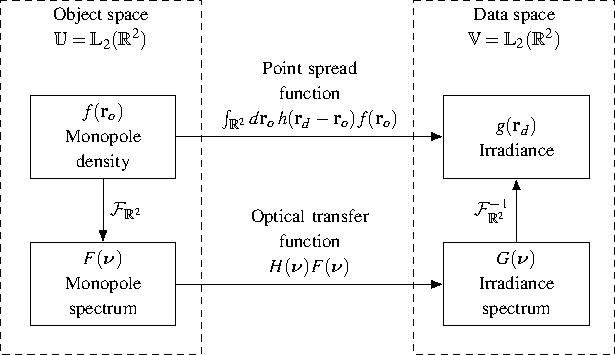
\includegraphics[scale=1.0]{../figures/monopole-block/monopole-block.pdf}
  \caption{The mapping between the object and data space of a monopole
    fluorescence microscope can be computed in two different bases---a delta
    function basis and a spatial harmonic basis. The change of basis is given by
    the two-dimensional Fourier transform denoted $\mathcal{F}_{\mbb{R}^2}$.}
     \label{fig:monopole-block}      
\end{figure}

The mapping between the object and the data in linear shift-invariant
microscopes takes a particularly simple form in a spatial harmonic basis. If we
apply the Fourier convolution theorem to Eq. \ref{eq:lsi} we find that
\begin{align}
  G(\bs{\nu}) = H(\bs{\nu})F(\bs{\nu}),\label{eq:freq}
\end{align}
where we define the \textit{scaled irradiance spectrum} as
\begin{align}
  G(\bs{\nu}) = \int_{\mbb{R}^2}d\mb{r}\, g(\mb{r})\, \text{exp}(-2\pi i\mb{r}\cdot\bs{\nu}),
\end{align}
the \textit{optical transfer function} as
\begin{align}
  H(\bs{\nu}) = \int_{\mbb{R}^2}d\mb{r}\, h(\mb{r})\, \text{exp}(-2\pi i\mb{r}\cdot\bs{\nu}),\label{eq:otf}
\end{align}
and the \textit{monopole spectrum} as
\begin{align}
    F(\bs{\nu}) = \int_{\mbb{R}^2}d\mb{r}\, f(\mb{r})\, \text{exp}(-2\pi i\mb{r}\cdot\bs{\nu}).
\end{align}
The point spread function is normalized and real-valued, so we know that the
optical transfer function is normalized $H(0) = 1$ and conjugate-symmetric
$H(-\bs{\nu}) = H^*(\bs{\nu})$.

Notice that Eqs. \ref{eq:lsi} and \ref{eq:freq} are expressions of the same
mapping between object and data space in different bases. Figure
\ref{fig:monopole-block} summarizes the relationship between object and data
space in both bases.

\subsubsection{Monopole coherent transfer functions}

\subsection{Dipole imaging in different bases}\label{sec:dipole}
Now we consider a microscope imaging a field of in-focus dipoles by recording
the irradiance on a two-dimensional detector. A function that assigns a real
number to each point on a plane is not sufficient to specify a field of dipoles
because the dipoles can have different orientations. To represent the object we
need to extend object space to $\mbb{U} = \mbb{L}_2(\mbb{R}^2\times\mbb{S}^2)$
where $\mbb{S}^2$ is the two-dimensional sphere (the usual sphere embedded in
$\mbb{R}^3$).

In a delta function basis the object can be represented by a function
$f(\ro, \so)$ called the \textit{spatio-angular dipole density}---the number of
dipoles at position $\ro{}$ per unit area oriented along $\so{}$ per unit solid
angle. Similar to the monopole case, we model the mapping between the object and
the irradiance in a delta function basis as an integral transform
\begin{align}
  g'(\rd') = \int_{\mbb{S}^2}d\so\int_{\mbb{R}^2}d\ro\, h'(\rd', \ro, \so)f(\ro, \so). 
\end{align}
where $h'(\rd', \ro, \so)$ is the irradiance at position $\rd'$ created by a
point source at $\ro$ with orientation $\so$. Once again, many fluorescence
microscopes can be modeled as magnifiers with shift-invariant blur
\begin{align}
  g'(\rd') = \int_{\mbb{S}^2}d\so\int_{\mbb{R}^2}d\ro\, h'(\rd' - m\ro, \so)f(\ro, \so). 
\end{align}

We define the same demagnified detector coordinate $\rd = \rd'/m$ and a new
normalization factor that corresponds to the total power incident on the
detector due to a spatial point source with an angularly uniform distribution of
dipoles
$P_\text{dip} = \int_{\mbb{S}^2}d\mb{s}\int_{\mbb{R}^2}d\mb{r}\, h'(m\mb{r},
\mb{s})$. We use these scaling factors to define the
\textit{orientation-dependent point spread function} as
\begin{align}
  h(\rd - \ro, \mb{s}) = \frac{h'(m[\rd - \ro], \mb{s})}{P_\text{dip}}, 
\end{align}
and the \textit{scaled irradiance} as 
\begin{align}
  g(\rd) = \frac{g'(m\rd)}{P_\text{dip}}. 
\end{align}
With these definitions we can express the mapping between the object and the
data as an integral over the sphere with a spatial convolution at each point
\begin{align}
g(\rd{}) = \int_{\mbb{S}^2}d\so{}\int_{\mbb{R}^2}d\ro{}\, h(\rd{} -\ro{}, \so{})f(\ro, \so). \label{eq:odpsf}
\end{align}
Similar to the monopole case, we have chosen to normalize the orientation-dependent point spread function so that
\begin{align}
  \int_{\mbb{S}^2}d\mh{s}\int_{\mbb{R}^2}d\mb{r}\, h(\mb{r}, \mh{s}) = 1. 
\end{align}
The orientation-dependent point spread function is a measurable quantity, so it
is real-valued and positive.

\subsubsection{Orientation-dependent optical transfer function}
We can make our first change of basis by applying the Fourier-convolution
theorem to Eq. \ref{eq:odpsf} which yields
\begin{align}
G(\bs{\nu}) = \int_{\mbb{S}^2}d\mh{s}\, H(\bs{\nu}, \mh{s})F(\bs{\nu}, \mh{s}) \label{eq:odotf},
\end{align}
where we define the \textit{orientation-dependent optical transfer function} as
  \begin{align}
  H(\bs{\nu}, \mh{s}) &= \int_{\mbb{R}^2}d\mb{r}\, h(\mb{r}, \mh{s})\, \text{exp}(-2\pi i\mb{r}\cdot\bs{\nu}),
  \end{align}
and the \textit{spatial dipole spectrum} as
  \begin{align}
  F(\bs{\nu}, \mh{s}) &= \int_{\mbb{R}^2}d\mb{r}\, f(\mb{r}, \mh{s})\, \text{exp}(-2\pi i\mb{r}\cdot\bs{\nu}). 
  \end{align}
  Since the orientation-dependent point spread function is normalized and real,
  we know that the orientation-dependent optical transfer function is normalized
  $\int_{\mbb{S}^2}d\mh{s}\, H(0, \mh{s}) = 1$ and conjugate-symmetric
  $H(-\bs{\nu}, \mh{s}) = H^*(\bs{\nu}, \mh{s})$.
  
  This choice of basis is well suited for simulating and analyzing objects that
  are angularly sparse and spatially dense.

  \begin{figure}
  \hspace{-5em}
  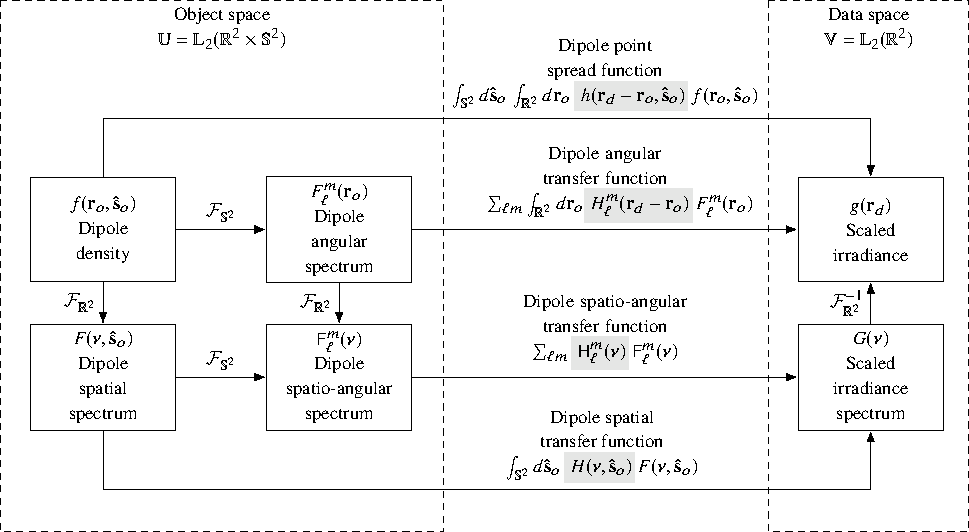
\includegraphics[scale=1.0]{../figures/dipole-block/dipole-block.pdf}
  \caption{The mapping between the object and data space of a dipole
    fluorescence microscope can be computed in four different bases---a delta
    function basis, a spatial-harmonic/angular-delta basis, a
    spatial-delta/spherical-harmonic basis, and a spatio-angular harmonic basis.
    The changes of basis are given by the two-dimensional Fourier transform
    denoted $\mathcal{F}_{\mbb{R}^2}$ and the spherical Fourier transform
    denoted $\mathcal{F}_{\mbb{S}^2}$.}
   \label{fig:dipole-block}      
    \end{figure}

\subsubsection{Angular transfer function}
The spherical harmonics are another set of convenient basis functions. We can
change basis from spherical delta functions to spherical harmonics by applying
the generalized Plancharel theorem for spherical functions
\begin{align}
  \ints{2}d\mh{s}{}\, p(\mh{s})q(\mh{s}) = \lmsum P_\ell^m Q_\ell^m, \label{eq:plan}
\end{align}
where $p(\mh{s})$ and $q(\mh{s})$ are arbitrary functions on the sphere and
\begin{align}
  P_\ell^m = \int_{\mbb{S}^2}d\mh{s}\, p(\mh{s})Y_\ell^{m*}(\mh{s}), 
\end{align}
is the spherical Fourier transform of $p(\mh{s})$ and $Y_{\ell}^m(\mh{s})$ are
the spherical harmonic functions defined in Appendix \ref{sec:sph}. Eq.
\ref{eq:plan} expresses the fact that scalar products are invariant under a
change of basis (see Eq. 3.78 of \cite{barrett2004}). The left-hand side of Eq.
\ref{eq:plan} is the scalar product of $\mbb{L}_2(\mbb{S}^2)$ functions in a
delta function basis and the right hand side is the scalar product of
$\mbb{L}_2(\mbb{S}^2)$ functions in a spherical harmonic function basis.
Applying Eq. \ref{eq:plan} to Eq. \ref{eq:odpsf} yields
\begin{align}
  g(\rd) = \lmsum H_\ell^m(\rd - \ro)F_\ell^m(\ro) \label{eq:atf-form}
\end{align}
where we have defined the \textit{angular transfer function} as
\begin{align}
  H_\ell^m(\mb{r}) = \int_{\mbb{S}^2}d\mh{s}\, h(\mb{r}, \mh{s})Y_{\ell}^{m*}(\mh{s}),\label{eq:atf-prep} 
\end{align}
and the \textit{angular dipole spectrum} as
\begin{align}
  F_\ell^m(\mb{r}) = \int_{\mbb{S}^2}d\mh{s}\, f(\mb{r}, \mh{s})Y_{\ell}^{m*}(\mh{s}).
\end{align}
Since the orientation-dependent point spread function is normalized and
real-valued, we know that the angular transfer function is normalized
$\int_{\mbb{R}^2}d\mb{r}\, H_0^0(\mb{r}) = 1$ and conjugate symmetric
$H_\ell^{-m}(\mb{r}) = (-1)^mH_\ell^{m*}(\mb{r})$.

This basis is well suited for simulating and analyzing objects that are
spatially sparse and angularly dense.

\subsubsection{Spatio-angular transfer function}
We can arrive at our final basis in two ways: by applying the generalized
Plancharel theorem for spherical functions to Eq. \ref{eq:odotf} or by applying
the Fourier convolution theorem to Eq. \ref{eq:atf-form}. We follow the
second path and find that
\begin{align}
G(\bs{\nu}) = \lmsum \msf{H}_\ell^m(\bs{\nu})\msf{F}_\ell^m(\bs{\nu}) \label{eq:saft},
\end{align}
where we have defined the \textit{spatio-angular transfer function} as
  \begin{align}
  \msf{H}_\ell^m(\bs{\nu}) &= \int_{\mbb{S}^2}d\mh{s}\, H(\bs{\nu}, \mh{s})Y_\ell^{m*}(\mh{s}),
  \end{align}
  and the \textit{spatio-angular dipole spectrum} as
  \begin{align}
  \msf{F}_\ell^m(\bs{\nu}) &= \int_{\mbb{S}^2}d\mh{s}\, F(\bs{\nu}, \mh{s})Y_\ell^{m*}(\mh{s}).
  \end{align}
  Since the orientation-dependent point spread function is normalized and
  real-valued, we know that the spatio-angular transfer function is normalized
  $\msf{H}_0^0(0) = 1$ and conjugate symmetric
  $\msf{H}_\ell^{-m}(-\bs{\nu}) = (-1)^m\msf{H}_\ell^{m*}(\bs{\nu})$.
  
  This basis is well suited for simulating and analyzing arbitrary samples
  because it exploits the sparsity of the imaging system. We will see this
  advantage explicitly in Section XXX when we calculate a specific
  spatio-angular transfer function and see that it has an angular band limit.

  Figure \ref{fig:dipole-block} summarizes the relationship between the four
  bases that we can use to compute the image of a field of dipoles. We reiterate
  that all four bases may be useful depending on the sparsity of the sample.
    
\subsubsection{Dipole coherent transfer functions}
Two-dimensional Fourier transforms and spherical Fourier transforms are the only
operations required to change between the transfer functions. However, there is
a well-known alternative for calculating optical transfer functions in terms of
coherent transfer functions. The key idea is that the orientation-dependent
point spread function can always be written as the absolute square of a
vector-valued function called the \textit{orientation-dependent coherent spread
  function}
\begin{align}
  h(\mb{r}, \mh{s}) = |\mb{c}(\mb{r}, \mh{s})|^2. \label{eq:absquare}
\end{align}
Physically, this decomposition corresponds to the fact that the irradiance is
always the absolute square of a vector-valued electric field.

Since the orientation-dependent transfer function is given by the
two-dimensional Fourier transform of the orientation-dependent point spread
function
\begin{align}
  H(\bs{\nu}) = \int_{\mbb{R}^2}d\mb{r}\,h(\mb{r}, \mh{s})\,\text{exp}[-2\pi i\mb{r}\cdot\bs{\nu}],
\end{align}
we can plug in Eq. \ref{eq:absquare} and use the autocorrelation theorem to
rewrite as
\begin{align}
  H(\bs{\nu}) = \int_{\mbb{R}^2}d\bs{\tau}\,\mb{C}(\bs{\tau}, \mh{s})\mb{C}^\dagger(\bs{\tau} - \bs{\nu}, \mh{s}), 
\end{align}
where the \textit{orientation-dependent coherent transfer function}
$\mb{C}(\bs{\tau}, \mh{s})$ is the two-dimensional Fourier transform of the
orientation-dependent coherent spread function
\begin{align}
  \mb{C}(\bs{\tau}, \mh{s}) = \int_{\mbb{R}^2}d\mb{r}\, \mb{c}(\mb{r}, \mh{s})\,\text{exp}[-2\pi i\mb{r}\cdot\bs{\tau}].
\end{align}
The relationships between all six transfer function are shown in Figure
\ref{fig:transfer-functions}. Note that we could define coherent equivalents for
all four incoherent transfer functions, but we restrict ourselves to these two
since they are the useful for our calculations.

\begin{figure}
  \hspace{-2em}
  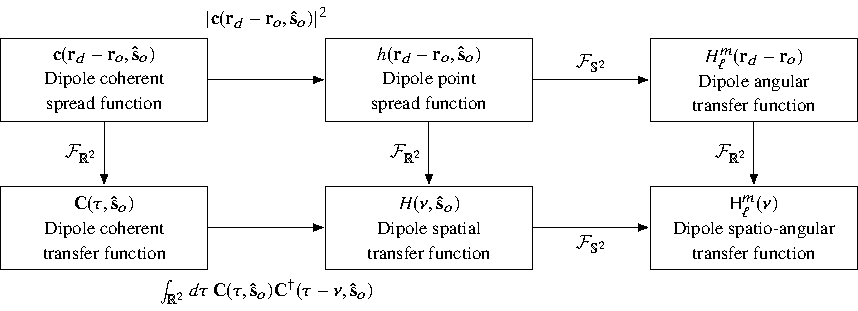
\includegraphics[scale=1.0]{../figures/transfer-functions/transfer-functions.pdf}
  \caption{There is one incoherent transfer function for each set of
    object-space basis functions, and these transfer functions are related by
    two-dimensional and spherical Fourier transforms---see center and right
    columns. There are an additional pair of coherent transfer functions that
    are useful for calculating the point spread function and optical transfer
    function---see left column.}
   \label{fig:transfer-functions}
 \end{figure}
    
    
\section{Results}\label{sec:results}
In this section we apply the tools we developed in the previous sections to
analyze a paraxial epi-fluorescence microscope. We start by reviewing the
derivation of the monopole point spread function in preparation for the
derivation of the orientation-dependent point spread function. We conclude the
section by analyzing the dipole imaging map in the four bases we described
earlier.

TODO: Define and discuss paraxial. 4f, illumination uniformity and ignoring in
monopole Where are excitation and detection dipoles parallel.

\subsection{Monopole point spread function of a paraxial epi-fluorescence microscope}
In this section we derive the form of the monopole point spread function
$h(\rd - \ro)$. First, we place a monopole emitter at the focal point of an
objective lens and calculate the field $U_{\text{bfp}}(\rb)$ created in the back
focal plane. We can model a paraxial thin lens as a quadratic phase element, so
it converts an incident spherical wave to a plane wave in the back focal plane
with a sharp cutoff at the exit pupil of the lens
\begin{align}
  U_{\text{bfp}}(\mb{r}_b) \propto \Pi\left(\frac{|\mb{r}_b|}{2\alpha}\right) \equiv
  \begin{cases}
    1\quad \text{if}\quad |\mb{r}_b| < \alpha,\\
    0\quad \text{else},
  \end{cases}
\end{align}
where $\rb$ is the two-dimensional coordinate in the back focal plane and
$\alpha$ is the collection half angle---see Figure XXX. 

A central result of Fourier optics is that the fields one focal distance from
either side of a paraxial lens are related by a scaled two-dimensional Fourier
transform. If we place a detector in the focal plane of the tube lens, then the
field on the detector $U_{\text{det}}(\mb{r}_d)$ is given by
\begin{align}
  U_{\text{det}}(\mb{r}_d) \propto \frac{J_1(k\alpha|\mb{r}_d|)}{|\mb{r}_d|}.
\end{align}
where $J_n(x)$ denotes the Bessel function of the first kind of order $n$, and
$k = 2\pi/\lambda$ is the wave number.

Finally, the detector measures the irradiance instead of the field, so we take
the modulus squared of the field to find that the measurable irradiance created
by a single monopole radiator at the origin is the familiar Airy disk
\begin{align}
  h(\mb{r}_d, \ro = 0) \propto |U_{\text{det}}(\mb{r}_d)|^2 = \left[\frac{J_1(k\alpha|\mb{r}_d|)}{|\mb{r}_d|}\right]^2.
\end{align}
Shifting the monopole in the transverse plane will introduce a linear phase
factor in the back focal plane which will manifest as a shift on the detector
due to the Fourier shift theorem. Therefore, the monopole imaging system is
shift invariant and we can rewrite the irradiance on the detector due to a
monopole at $\ro$ as
\begin{align}
  h(\rd, \ro) = h(\rd - \ro). \label{eq:shift}
\end{align}
We have modeled a microscope with unit magnification, but a similar point spread
function can be found for magnifying microscopes by making a change of
variables (see \cite{barrett2004}, section 7.2.7).

Rotating a monopole will leave its image unchanged. Therefore, our imaging
system is rotation invariant and we can simplify the orientation-dependent point spread function further with
\begin{align}
  h(\rd - \ro) = h(|\rd - \ro|). \label{eq:rotational}
\end{align}

\subsection{Orientation-dependent point spread function of a paraxial epi-fluorescence microscope}
In this section we will calculate the orientation-dependent point spread
function $h(\rd - \ro, \mh{s})$ of a paraxial epi-fluorescence microscope. We can
make our first simplifying step by realizing the excitation and detection
processes are incoherent, which means that the orientation-dependent PSF is
separable:
\begin{align}
  h(\rd, \ro, \so) = h_{\text{exc}}(\ro, \so)\,h_{\text{det}}(\rd, \ro, \so). \label{eq:kernelsep}
\end{align}
We can calculate the excitation and detection terms separately then take their
product to find the complete orientation-dependent point spread function.

\subsubsection{Orientation-dependent excitation model}
When we developed the monopole imaging model we ignored the excitation process
because we excited the fluorophores with a spatially uniform excitation beam and
monopoles have no orientation dependence. For the dipole imaging model we must
model the excitation process because the excitation process is rarely angularly
uniform (carefully calibrated TIRF systems are an exception).

In this section we will calculate the excitation kernel
$h_{\text{exc}}(\ro, \so)$ for the paraxial epi-illumination microscope under
unpolarized (TODO: Define/cite) K\"{o}ehler illumination shown in Figure
\ref{fig:exccoords}. We will only consider spatially uniform excitation, so the
excitation kernel will not depend on $\ro$
\begin{align}
  h_{\text{exc}}(\ro, \so) = h_{\text{exc}}(\so).
\end{align}
We can interpret $h_{\text{exc}}(\so)$ as the relative probability of exciting a
molecule with dipole orientation $\so$. Our approach is similar to previous work
\cite{fourkas2001, chandler2017}, but here we consider paraxial, incoherent, and
unpolarized illumination (TODO improve).

\begin{figure}[h]
 \centering
   \centering
   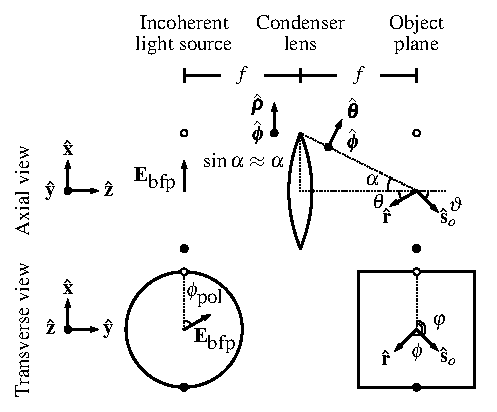
\includegraphics[scale=.9]{../figures/excitation-coords/excitation-coords.pdf}
   \caption{Illumination geometry and coordinates for a paraxial epifluorescence
     microscope. An unpolarized and incoherent light source (or its image) is in
     the back focal plane of the condenser lens.}
   \label{fig:exccoords}
 \end{figure}

We start by expressing the dipole moment $\so{}$ in Cartesian coordinates
\begin{align}
  \so{} &= s_x\mh{x} + s_y\mh{y} + s_z\mh{z}. \label{eq:spherical}
\end{align}
We place the dipole in the focal plane of an aplanatic and
polarization-preserving objective lens with its optical axis aligned with the
$\mh{z}$ axis. Next, we place a spatially incoherent, spatially uniform,
unpolarized light source (or its image) in the back aperture of the objective
lens to illuminate the focal plane. In this geometry each point in the back
focal plane generates a plane wave that illuminates the sample.

To model the unpolarized light source we will use polarized ray tracing
\cite{foreman2011} to find the response for a single polarized ray, then
integrate over the rays and all polarizations to find the complete response.
First, we model the electric field at every point on the back focal plane as
\begin{align}
   \mb{E}_{\text{bfp}}(\phi_{\text{pol}}) &\propto \cos\phi_{\text{pol}}\mh{x} + \sin\phi_{\text{pol}}\mh{y}, \label{eq:bfp0}
\end{align}
where $\phi_{\text{pol}}$ is the polarization orientation and \{$\mh{x}$,
$\mh{y}$\} are transverse Cartesian basis vectors. Note that Eq. \ref{eq:bfp0}
describes the incoherent electric fields at every point in the back focal
plane--- it does not describe a coherent plane wave. To find the electric field
immediately after the paraxial lens we apply a position-dependent rotation
matrix (see the rotation matrices in \cite{foreman2011, backer2014} under the
paraxial approximation):

\begin{align}
  \mb{E}_{\text{ff}}(\theta, \phi, \phi_{\text{pol}}) & \propto 
  \begin{bmatrix}
    1 & 0 &\theta \cos\phi\\
    0 & 1 &\theta \sin\phi\\
    -\theta\cos\phi&-\theta \sin(\phi)&1
  \end{bmatrix}
  \begin{bmatrix}
    \cos\phi_{\text{pol}}\\
    \sin\phi_{\text{pol}}\\
    0
  \end{bmatrix},\\
  \intertext{so that}
  \mb{E}_{\text{ff}}(\theta, \phi, \phi_{\text{pol}}) &\propto \cos\phi_{\text{pol}}\mh{x} + \sin\phi_{\text{pol}}\mh{y} - \theta\cos(\phi - \phi_{\text{pol}})\mh{z}.\label{eq:eff}
\end{align}
The probability that a dipole oriented along $\so{}$ is excited by a ray with
electric field $\mb{E}$ is given by 
\begin{align}
  |\mb{E}_{\text{ff}}(\theta, \phi, \phi_{\text{pol}}) \cdot \so{}|^2 \propto s_x^2\cos^2\phi_{\text{pol}} + s_y^2\sin^2\phi_{\text{pol}} + s_z^2\theta^2\cos^2(\phi - \phi_{\text{pol}}). \label{eq:integrand}
\end{align}
To find the complete excitation kernel we need to integrate Eq.
\ref{eq:integrand} over all polarization orientations and rays:
\begin{align}
  h_{\text{exc}}(\so{}) \propto \int_0^{\alpha}\theta d\theta\int_0^{2\pi}d\phi\int_0^{2\pi}d\phi_{\text{pol}}\, |\mb{E}_{\text{ff}}(\theta, \phi, \phi_{\text{pol}}) \cdot \so{}|^2. \label{eq:integral}
\end{align}
Plugging Eq. \ref{eq:integrand} into Eq. \ref{eq:integral}, evaluating the
integrals, and dropping constants gives
\begin{align}
  h_{\text{exc}}(\vartheta) &\propto s_x^2 + s_y^2 + \frac{1}{2}\alpha^2s_z^2.
\end{align}
We can rewrite the excitation kernel in terms of a single variable with the
substitutions $s_x^2 + s_y^2 = \sin^2\vartheta$ and $s_z^2 = \cos^2\vartheta$:
\begin{align}
  h_{\text{exc}}(\vartheta) &\propto \sin^2\vartheta + \frac{1}{2}\alpha^2\cos^2\vartheta \label{eq:hexctheta}.
\end{align}

Figure \ref{fig:excitation} shows the excitation response as a function of
inclination angle $\vartheta$ and excitation half angle $\alpha$. The largest
variation of the excitation kernel occurs when the maximum excitation angle is
zero---plane-wave illumination. As $\alpha$ grows, dipoles parallel to the optic
axis are more likely to be excited and the variation of the excitation kernel
decreases.
\begin{figure}[h]
 \centering
   \centering
   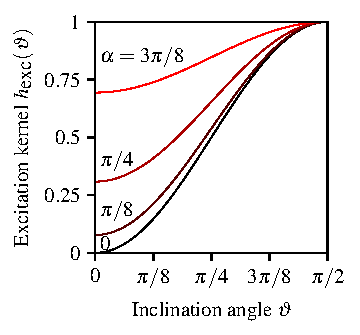
\includegraphics[scale=0.95]{../figures/excitation/excitation.pdf}
   \caption{Dipole excitation kernel $h_{\text{exc}}(\vartheta)$ as a function of
     inclination angle $\vartheta$ and excitation half angle $\alpha$.}
   \label{fig:excitation}
 \end{figure}

 \subsubsection{Orientation-dependent dipole detection model}
 In this section we will calculate the detection kernel of an epi-detection
 microscope---the irradiance on the detector due to a single dipole with fixed
 position and orientation. [TODO Improve] Our approach mimics existing work
 \cite{backer2014, nov2006, agrawal2012}, but we restrict ourselves to the
 paraxial approximation.

\begin{figure}[h]
 \centering
   \centering
   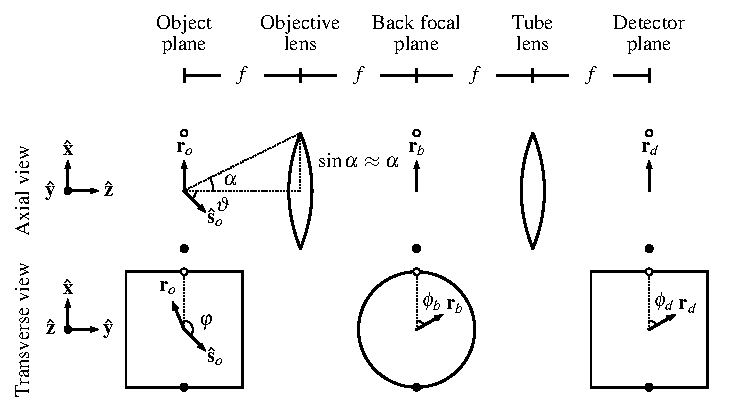
\includegraphics[scale=.9]{../figures/detection-coords/detection-coords.pdf}
   \caption{Detection geometry and coordinates. We calculate the detection
     kernel $h_{\text{det}}(\rd, \ro, \so)$ for a paraxial 4$f$ imaging
     system.}
   \label{fig:detection}
 \end{figure}
 
We consider a single dipole emitter at the origin with a fixed dipole emission
moment oriented along $\so{}$. The electric field at a position $\mb{r}$ far
from the dipole is given by
\begin{align}
  \mb{E}_{\text{ff}}(\mb{r}, \so{}) \propto \frac{\text{exp}[ik|\mh{r}|]}{|\mh{r}|}\mh{r} \times \so{} \times \mh{r}. \label{eq:ff}
\end{align}
We place the dipole in the focal plane of the same 4$f$ imaging system we
considered in the monopole case---see Figure \ref{fig:detection}. The dipole emits
spherical wavefronts so we can reuse our argument for shift invariance and drop
the phase dependence of the electric field
\begin{align}
  \mb{E}_{\text{ff}}(\mb{r}, \so{}) \propto \mh{r} \times \so{} \times \mh{r} \label{eq:ff2}
\end{align}
We also note that we can rewrite a shift-invariant kernel as
\begin{align}
h_{\text{det}}(\rd, \ro, \so) = h_{\text{det}}(\rd - \ro, \so), 
\end{align}
which will simplify our derivation---we only need to calculate the response for
a dipole positioned along the optic axis. We can rewrite the cross products in terms
of a matrix multiplication
\begin{align}
  \mb{E}_{\text{ff}}(\mb{r}, \so{}) \propto [\tensor{I} - \mh{r}\mh{r}^{\dagger}]\so,
\end{align}
where $\tensor{I}$ is a $3\times 3$ identity matrix. If we place the molecule in
the focal plane of an aplanatic and polarization-preserving objective lens with
the lens' optical axis aligned with the $\mh{z}$ axis, then we can find the
electric field in the back focal plane by multiplying the electric field with a
position-dependent rotation matrix and truncating waves outside the detection
collection half angle $\alpha$
\begin{align}
  \mb{E}_{\text{bfp}}(\mb{r}, \so{}) \propto \mb{R}_{\text{obj}}(\mh{r})[\tensor{I} - \mh{r}\mh{r}^{\dagger}]\so\Pi\left(\frac{\theta}{2\alpha}\right).
\end{align}
After plugging in paraxial positions
\begin{align}
  \mh{r}(\theta,\phi) \approx \theta\cos\phi\mh{x} + \theta\sin\phi\mh{y} + \mh{z},
\end{align}
and the paraxial rotation matrix
\begin{align}
  \mb{R}_{\text{obj}}(\theta, \phi) &=
  \begin{bmatrix}
    1 & 0 &-\theta \cos\phi\\
    0 & 1 &-\theta \sin\phi\\
    -\theta\cos\phi&-\theta \sin(\phi)&1
  \end{bmatrix},
\end{align}
then dropping the $\theta^2$ $\mh{z}$ components and changing from spherical
coordinates to cylindrical coordinates by substituting $(r_b, \phi_b)$ for
$(\theta, \phi)$ we find that
\begin{align}
  \mb{E}_{\text{bfp}}(r_b, \phi_b, \so{}) \propto \left\{\left[s_x - s_zr_b\cos\phi_b\right]\mh{x} + \left[s_y - s_z r_b\sin\phi_b\right]\mh{y}\right\}\Pi\left(\frac{r_b}{2\alpha}\right). \label{eq:bfp2}
\end{align}
Equation \ref{eq:bfp2} is easier to work with if we introduce the radial vector
field $\mh{\bs{\rho}} = \cos\phi_b\mh{x} + \sin\phi_b\mh{y}$ and rewrite as
\begin{align}
  \mb{E}_{\text{bfp}}(r_b, \phi_b, \so{}) \propto \left\{s_x\mh{x} + s_y\mh{y} - s_z r_b \mh{\bs{\rho}}\right\}\Pi\left(\frac{r_b}{2\alpha}\right). \label{eq:bfp3}
\end{align}
Equation \ref{eq:bfp3} shows that the transverse components of the dipole
($s_x, s_y$) create linear vector fields in the back focal plane
($\mh{x}, \mh{y}$) while the axial component of the dipole $s_z$ creates a radial
vector field in the back focal plane $\mh{z}$. 

We complete the 4$f$ system by placing a tube lens one focal length from the
back focal plane and a planar detector---see Figure \ref{fig:detection}. Under
the paraxial approximation we can find the electric field in the detector plane
by taking the Fourier transform of the field in the back focal plane
\cite{goodman1996}
\begin{align}
  \mb{E}_{\text{det}}(\rd{}, \so{}) &= \int_{\mbb{R}^2}d\rb{} \mb{E}_{\text{bfp}}(\rb{})\, \text{exp}\left[ik\,\rb{}\cdot\rd{}\right].\label{eq:det1}
\end{align}
We evaluate the integral in Appendix \ref{sec:ftvec} and show that 
\begin{align}
  \mb{E}_{\text{det}}(r_d, \so{}) \propto \frac{J_1(k\alpha r_d)}{r_d}s_x\mh{x} + \frac{J_1(k\alpha r_d)}{r_d}s_y\mh{y} - i\alpha\frac{J_2(k\alpha r_d)}{r_d}s_z\mh{\bs{\rho}}.
\end{align}
Once again we find that the transverse component of the dipole creates a linear
field and the axial component of the dipole creates a radial field, but on the
detector the linear and radial fields are out of phase by $\pi/2$. This crucial
phase factor is a direct consequence of the fact that the linear fields are real
and even---the Fourier transform of a real and even function is real and
even---and the radial fields are real and odd---the Fourier transform of a real
and odd function is imaginary and odd.

Our final step is to calculate the irradiance on the detector
\begin{align}
  h_{\text{det}}(r_d, \so{}) &\propto |\mb{E}_{\text{det}}(r_d, \so{})|^2.
\end{align}
The irradiance is the sum of the contributions from the linear and radial fields
since their fields are out of phase, so
\begin{align}
  h_{\text{det}}(r_d, \vartheta) &\propto a_1(r_d)\sin^2\vartheta + \frac{1}{2}\alpha^2 a_2(r_d)\cos^2\vartheta, 
\end{align}
where we have defined
\begin{align}
  a_n(r_d) \equiv \frac{n}{\pi}\left[\frac{J_n(k\alpha r_d)}{r_d}\right]^2. 
\end{align}
Notice that we retain the $\alpha^2$ irradiance term even though we dropped
$\theta^2$ electric field terms since these terms would become $\theta^4$
irradiance terms.

Figures \ref{fig:hdet} and \ref{fig:microscope} summarize the most important
features of the dipole detection model. When $\alpha$ is very small the
detection kernel is the usual Airy pattern weighted by $\sin^2\vartheta$. Note
that the monopole detection model ignores the $\sin^2\vartheta$ dependence---see
Figure \ref{fig:microscope} a) and b). As $\alpha$ grows, the relative
contribution of the higher-order Airy pattern increases. The most important
result is that the dipole detection model is not separable into the product of a
spatial and angular kernel---even under the paraxial approximation. The
detection model is only separable when $\alpha$ approaches zero, which is almost
never the case in real microscopes. We refer to the non-separability of the
detection kernel as \textit{spatio-angular coupling} because the orientation of
the dipole is coupled to the spatial pattern of irradiance on the detector.

The paraxial detection kernel is rotationally symmetric---it depends on $r_d$ instead of
$\rd$. This symmetry is a result of the $\pi/2$ phase shift between the linear
and radial fields on the detector. If the phase shift between the linear and
radial fields was not exactly $\pi/2$ then the fields would interfere on the
detector, and we would lose rotational symmetry. Tracing back further, the
rotational symmetry is due to the fact that the field in the back focal plane
could be written as a sum of a linear and radial field which is only true under
the paraxial approximation---the rotational symmetry of the detection kernel is
only true to first order. Despite the approximation, we still feel that the
rotational symmetry of the detection kernel is a valuable result since it helps
build an intuition about the dominant effects outside the paraxial
approximation. 

Note that we have restricted our analysis to an imaging system with unit
magnification. We will continue with this simplification and mention that an
imaging system with an arbitrary magnification can be modeled using the model
for a system with unit magnification and a change of variable (see
\cite{barrett2004} section 7.2.7).

\begin{figure}[h]
 \centering
   \centering
   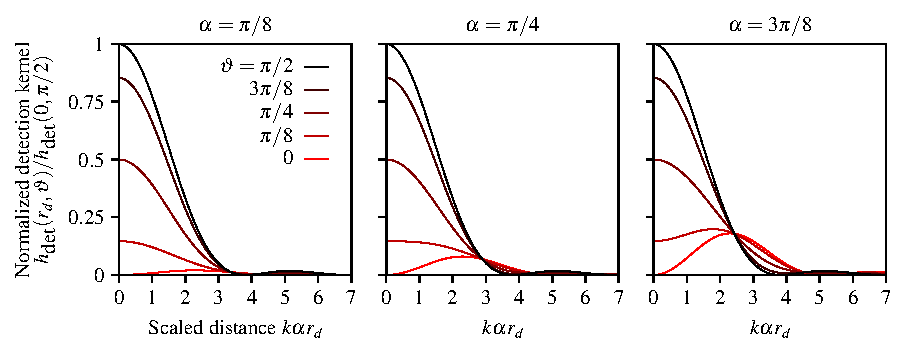
\includegraphics[scale=0.8]{../figures/detection/detection.pdf}
   \caption{Normalized detection kernel as a function of the scaled radial
     detection coordinate $k\alpha r_d$, the dipole inclination angle
     $\vartheta$, and the collection angle $\alpha$. For small
     collection angles (left) the detection kernel of axial dipoles
     (\textcolor{red}{\textbf{red}}) is small compared to transverse dipoles
     (\textbf{black}), but the relative contribution of axial dipoles increases
     with the collection angle (see \textcolor{red}{\textbf{red}} lines from
     left to right).}
   \label{fig:hdet}
 \end{figure}
 
\begin{figure}[h]
 % \captionsetup{width=1.0\linewidth}
 \centering
   \centering
   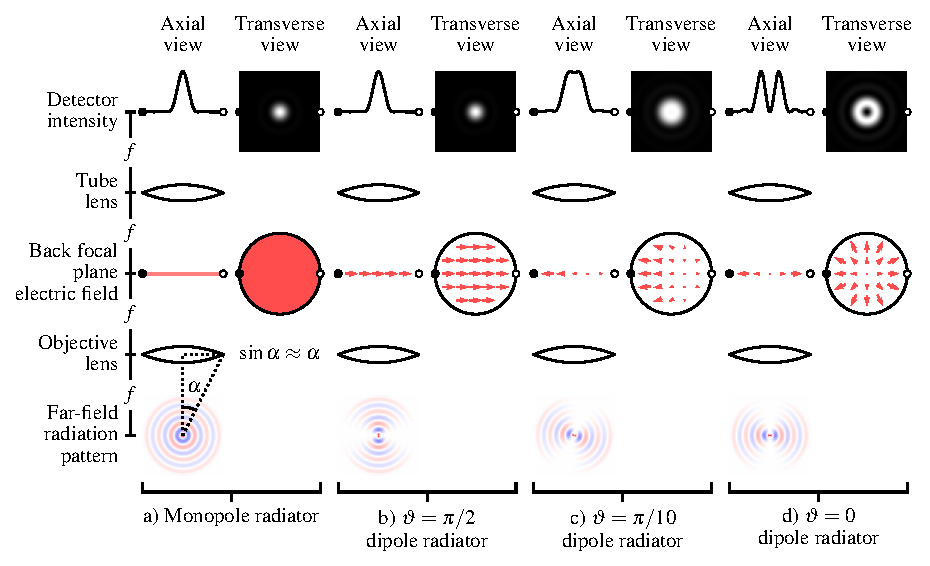
\includegraphics[scale=0.8]{../figures/microscope/microscope.pdf}
   \caption{Comparison of paraxial detection models for monopole radiators a)
     and dipole radiators b)--d). a) Monopole radiators fill the back focal
     plane with a uniform scalar field which gives rise to the familiar Airy
     disk on the detector. b) A transverse dipole radiator also creates an Airy
     disk, but the back focal plane is filled with a uniform vector field. c) An
     axial dipole radiator creates a radial electric field pattern in the back
     focal plane which creates a higher-order Airy disk on the detector. d)
     Dipoles that are not transverse or axial still create radially symmetric
     irradiance patterns under the paraxial approximation. Fields from
     transverse dipoles are real and even while fields from axial dipoles are
     real and odd which causes a relative $\pi/2$ phase shift for the fields on
     the detector. This phase shift means that the fields from transverse and
     axial components of the dipole do not interfere, which causes radially
     symmetric irradiance patterns.}
   \label{fig:microscope}
 \end{figure}

\subsubsection{Complete orientation-dependent point spread function}
 Combining the results of the previous two sections yields a simplified dipole
 imaging model 
 \begin{align}
g(\rd{}) = \int_{\mbb{S}^2}d\so{}\int_{\mbb{R}^2}d\ro{}\, h(|\rd - \ro|, |\so\cdot \mh{z}|)f(\ro, \so).\label{eq:simplified}
 \end{align}
 where we have written the kernel in terms of $|\so\cdot\mh{z}| = \cos\vartheta$
 to explicitly show the dependence on $\so$. In previous sections we showed that the
 kernel is given by 
 \begin{align}
   h(r, \vartheta) &\propto h_{\text{exc}}(\vartheta)h_{\text{det}}(r,\vartheta).
 \end{align}
 Plugging in our results we find:
 \begin{align}
   h(r, \vartheta) &\propto \left[\sin^2\vartheta + \frac{1}{2}\alpha^2 \cos^2\vartheta\right]\left[a_1(r)\sin^2\vartheta + \frac{1}{2}\alpha^2 a_2(r)\cos^2\vartheta\right]. \label{eq:sa-psf}
 \end{align}

 Comment on inversion/antipodal symmetry. 

 To demonstrate the orientation-dependent point spread function, we calculate
 the irradiance pattern created by a set of equally spaced dipoles with varying
 orientation given by
 \begin{align}
   f_{\text{(ph1)}}(x_o, y_o, \vartheta, \varphi) = \sum_{i=0}^3 \sum_{j=0}^3 \delta\left(x_o - \frac{i}{3}\right)\, \delta\left(y_o - \frac{j}{3}\right)\, \delta\left(\cos\vartheta - \cos\left(\frac{\pi i}{6}\right)\right)\, \delta\left(\varphi - \frac{2\pi j}{3}\right),\label{eq:phantom1}
 \end{align}
 where the subscript (ph1) indicates that this is the first phantom. To find the
 irradiance pattern we plug Eq. \ref{eq:phantom1} into Eq. \ref{eq:simplified}
 and use the sifting property
 \begin{align}
   g_{\text{(ph1)}}(x_d, y_d) = \sum_{i=0}^3 \sum_{j=0}^3 h\left(\sqrt{\left(x_d - \frac{i}{3}\right)^2 + \left(y_d - \frac{j}{3}\right)^2}, \frac{\pi i}{6}\right).\label{eq:phantom1irr}
 \end{align}
 
\subsection{Orientation-dependent optical transfer function of a paraxial epi-fluorescence microscope}\label{sec:trans}
  In Appendix \ref{sec:airy} we evaluate the 2D spatial Fourier transforms of
  $a_1(r)$ and $a_2(r)$ to find that
  \begin{align}
    H(\nu, \vartheta) &\propto \left[\sin^2\vartheta + \frac{1}{2}\alpha^2 \cos^2\vartheta\right]\left[A_1(\nu)\sin^2\vartheta + \frac{1}{2}\alpha^2 A_2(\nu)\cos^2\vartheta\right].
  \end{align}
  where 
\begin{align}
  A_1(\nu) &= \frac{2}{\pi}\left\{\cos^{-1}\left(\frac{\nu}{2\nu_o}\right) - \frac{\nu}{2\nu_o}\sqrt{1 - \left(\frac{\nu}{2\nu_o}\right)^2}\right\}\Pi\left(\frac{\nu}{4\nu_o}\right), \\
  A_2(\nu) &= \frac{2}{\pi}\Bigg\{\cos^{-1}\left(\frac{\nu}{2\nu_o}\right) - \left[3 - 2\left(\frac{\nu}{2\nu_o}\right)^2\right]\frac{\nu}{2\nu_o}\sqrt{1 - \left(\frac{\nu}{2\nu_o}\right)^2}\Bigg\}\Pi\left(\frac{\nu}{4\nu_o}\right).
\end{align}
The orientation-dependent optical transfer function is shown in Figure
\ref{fig:odotf}. The orientation-dependent transfer function has the usual
spatial-frequency cutoff at $\nu_c = 2\nu_o$ for all dipole orientations.

\begin{figure}[h]
 % \captionsetup{width=1.0\linewidth}
 \centering
   \centering
   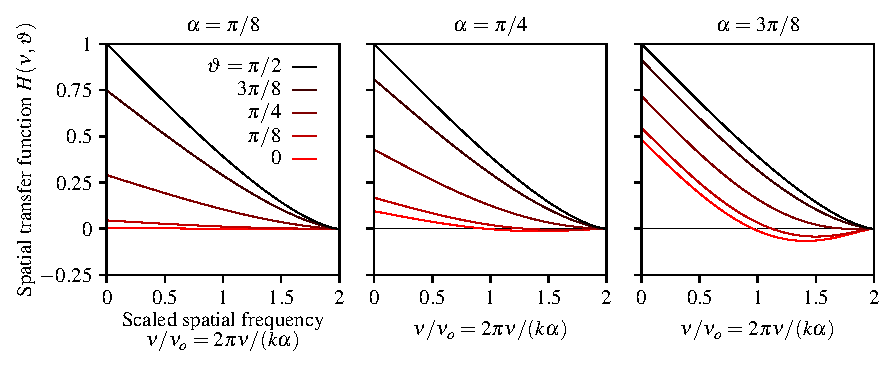
\includegraphics[scale=0.8]{../figures/stf/stf.pdf}
   \caption{Orientation-dependent transfer function as a function of the scaled
     spatial frequency, the dipole inclination angle $\vartheta$, and the
     collection angle $\alpha$. For small collection angles (left) the STF for
     axial dipoles (\textcolor{red}{\textbf{red}}) is small compared to
     transverse dipoles (\textbf{black}), but the relative contribution of axial
     dipoles increases with the collection angle (see
     \textcolor{red}{\textbf{red}} lines from left to right). The STF of axial
     dipoles is negative at high spatial frequencies because the central minimum
     of the axial kernel corresponds to the position of the dipole.
     Equivalently, a high-spatial-frequency pattern of axial dipoles will
     generate an irradiance pattern where the minimum irradiance corresponds to
     the peak of the axial dipole density.}
   \label{fig:odotf}
 \end{figure}

 To demonstrate the spatial transfer spread function, we calculate the
 irradiance pattern created by a set of equally spaced disks with varying radius
 containing fluorophores with varying orientation given by
 \begin{align}
   f_{\text{(ph2)}}(x_o, y_o, \vartheta, \varphi) = \sum_{i=0}^3 \sum_{j=0}^3 \Pi\left(\frac{10}{j}\sqrt{\left(x_o - \frac{i}{3}\right)^2 + \left(y_o - \frac{j}{3}\right)^2}\right) \delta\left(\cos\vartheta - \cos\left(\frac{\pi i}{6}\right)\right)\, \delta\left(\varphi - \frac{2\pi j}{3}\right).\label{eq:phantom2}
 \end{align}
 \begin{align}
   G_{\text{(ph2)}}(\nu_x, \nu_y) = \sum_{i=0}^3 \sum_{j=0}^3 H\left(\nu_x, \nu_y, \frac{\pi i}{6}, \frac{2\pi j}{3}\right)\left[\frac{j}{10\nu}J_1\left(\frac{2\pi j\nu}{10}\right)\right]\text{exp}\left(-2\pi i\left[\frac{i}{3}\nu_x + \frac{j}{3}\nu_y\right]\right).\label{eq:phantom2g}
 \end{align}
 Finally, we calculate the inverse Fourier transform of the irradiance spectrum
 to find the irradiance. 
 
 \subsection{Angular transfer function (ATF) of a paraxial epi-fluorescence microscope}
To calculate the angular transfer function we plug the spatio-angular point
spread function Eq. \ref{eq:sa-psf} into Eq. \ref{eq:atf-prep} and evaluate the
integrals using a computer algebra package \cite{meurer2017} to find
\begin{alignat}{6}
  H_l^m(r) \propto \quad 7&\{\hphantom{-}32&&a_1(r)&& + 4\alpha^2[a_1(r) + a_2(r)]&&+ 3\alpha^4a_2(r)\}&&\delta_{\ell 0}\delta_{m0}+\nonumber\\
  4\sqrt{5}&\{-16&&a_1(r)&& + \hphantom{1}\alpha^2[a_1(r) + a_2(r)] &&+ 3\alpha^4a_2(r)\}&&\delta_{\ell 2}\delta_{m0} + \nonumber\\
  8&\{\hphantom{-1}4&&a_1(r)&& - 2\alpha^2[a_1(r) + a_2(r)] &&+ \hphantom{1}\alpha^4a_2(r)\}&&\delta_{\ell 4}\delta_{m0}.
\end{alignat}
The degree $\ell$ and order $m$ of the non-zero terms in the ATF follow directly
from specific features of the kernel. First, the spatio-angular point spread
function is symmetric under inversion of the dipole moment. This symmetry is
maintained in the angular transfer function since all of the non-zero terms have
an even degree $\ell=0, 2, 4$, and the corresponding spherical harmonics
$Y_0^0(\so)$, $Y_2^0(\so)$, $Y_4^0(\so)$ are symmetric under inversion. Second,
we showed that under the paraxial approximation our kernel is rotationally
symmetric which allows us to write the kernel as a function of $r$ instead of
$\mb{r}$. This symmetry is maintained in the ATF since all of the non-zero terms
have order $m=0$. Finally, both the excitation and detection kernels are
degree-2 trigonometric polynomials, which implies that the maximum degree of the
spatio-angular point spread function is 4. This feature of the kernel appears in
the angular transfer function since only $\ell=0, 2$, and $4$ terms are
non-zero.

\begin{figure}[h]
 \centering
   \centering
   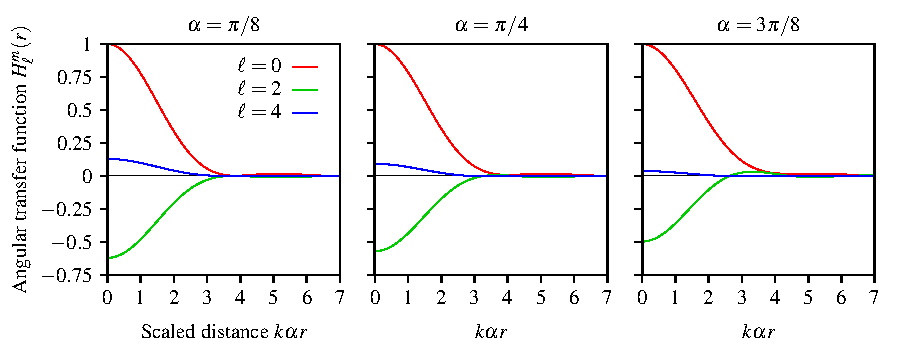
\includegraphics[scale=0.8]{../figures/atf/atf.pdf}
   \caption{ATF as a function of the scaled radial detection coordinate
     $k\alpha r$, the spherical harmonic degree $\ell$, and the collection angle
     $\alpha$. 
   }
   \label{fig:atf}
 \end{figure}

 To demonstrate the angular transfer function, we calculate the irradiance
 pattern created by a set of equally spaced fluorophore distributions with
 varying orientation and angular distribution given by
 \begin{align}
   f_{\text{(ph3)}}(x_o, y_o, \vartheta, \varphi) = \sum_{i=0}^3 \sum_{j=0}^3 \delta\left(x_o - \frac{i}{3}\right)\, \delta\left(y_o - \frac{j}{3}\right)\, f_{\text{(cone)}}\left(\vartheta, \varphi; \frac{\pi i}{6}, \frac{2\pi j}{3}, \frac{\pi i}{6}\right),\label{eq:phantom3}
 \end{align}
 where
 \begin{align}
   f_{\text{(cone)}}(\so; \so', \Delta) = f_{\text{(cone)}}(\vartheta, \varphi; \vartheta', \varphi', \Delta) = \frac{1}{4\pi(1 - \cos\Delta)}\Pi\left(\frac{\mh{s}\cdot\mh{s}'}{\cos\Delta}\right).
 \end{align}
 To calculate the irradiance pattern we calculate the angular density spectrum
 of the phantom (we calculate the spherical Fourier transform of the cone in
 Appendix \ref{sec:cone}), plug the result into Eq. XXX, then use the sifting
 property to find that
 \begin{align}
   g_{\text{(ph3)}}(x_d, y_d) = \sum_{\ell m}\sum_{i=0}^3 \sum_{j=0}^3 H_\ell^m\left(\sqrt{\left(x_d - \frac{i}{3}\right)^2 + \left(y_d - \frac{j}{3}\right)^2}\right) F_{\ell\text{(cone)}}^m\left(\frac{\pi i}{6}, \frac{2\pi j}{3}, \frac{\pi i}{6}\right),\label{eq:phantom3}
 \end{align}

\subsection{Spatio-angular transfer function (SATF)  of a paraxial epi-fluorescence microscope}
  \begin{alignat}{6}
  H_l^m(\nu) \propto \quad 7&\{\hphantom{-}32&&A_1(\nu)&& + 4\alpha^2[A_1(\nu) + A_2(\nu)]&&+ 3\alpha^4A_2(\nu)\}&&\delta_{\ell 0}\delta_{m0}+\nonumber\\
  4\sqrt{5}&\{-16&&A_1(\nu)&& + \hphantom{1}\alpha^2[A_1(\nu) + A_2(\nu)] &&+ 3\alpha^4A_2(\nu)\}&&\delta_{\ell 2}\delta_{m0} + \nonumber\\
  8&\{\hphantom{-1}4&&A_1(\nu)&& - 2\alpha^2[A_1(\nu) + A_2(\nu)] &&+ \hphantom{1}\alpha^4A_2(\nu)\}&&\delta_{\ell 4}\delta_{m0}.
\end{alignat}

\begin{figure}[h]
 \centering
   \centering
   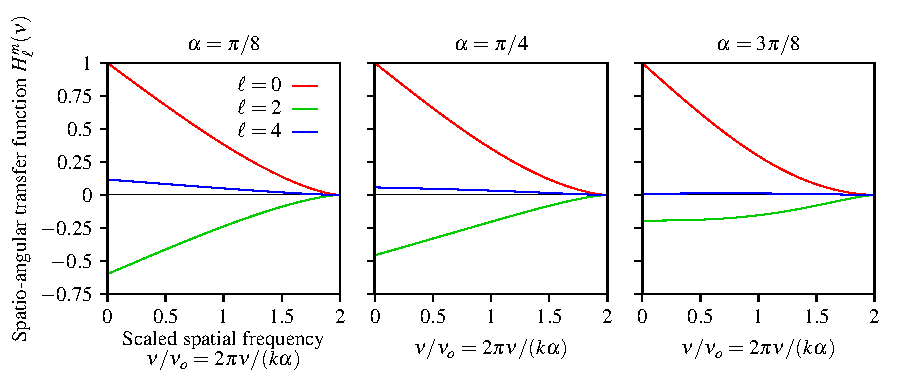
\includegraphics[scale=0.8]{../figures/satf/satf.pdf}
   \caption{SATF as a function of the scaled spatial frequency, the spherical
     harmonic degree $\ell$, and the collection angle $\alpha$. }
   \label{fig:atf}
 \end{figure}

 To demonstrate the spatio-angular transfer function, we calculate the
 irradiance pattern created by a set of equally spaced disks of fluorophores
 with varying radius and angular distribution given by
 \begin{align}
   f_{\text{(ph4)}}(x_o, y_o, \vartheta, \varphi) = \sum_{i=0}^3 \sum_{j=0}^3 \Pi\left(\frac{10}{j}\sqrt{\left(x_o - \frac{i}{3}\right)^2 + \left(y_o - \frac{j}{3}\right)^2}\right)f_{\text{(cone)}}\left(\vartheta, \varphi; \frac{\pi}{2}, 0, \frac{\pi i}{6}\right),\label{eq:phantom4}
 \end{align}
 To calculate the irradiance pattern created by the phantom we calculate the
 spatio-angular spectrum, plug the result into Eq. XXX, then take the inverse
 Fourier transform to find the irradiance.
  \begin{align}
    G_{\text{(ph2)}}(\nu_x, \nu_y) = \sum_{\ell m}\sum_{i=0}^3 \sum_{j=0}^3 H_\ell^m(\nu_x, \nu_y)\left[\frac{j}{10\nu}J_1\left(\frac{2\pi j\nu}{10}\right)\right]\text{exp}\left(-2\pi i\left[\frac{i}{3}\nu_x + \frac{j}{3}\nu_y\right]\right)F_{\ell\text{(cone)}}^m\left(\frac{\pi i}{6}, \frac{2\pi j}{3}, \frac{\pi i}{6}\right).\label{eq:phantom4g}
 \end{align}

 
\section{Discussion}\label{sec:discussion}
\subsection{Reconstructions}
Since the ATF effectively contains three OTFs it is tempting to conclude that
fluorescence microscopes pass three times as much information about the dipoles
as monopoles. This is not true. The microscope still only measures a single
member of $\mbb{L}_2(\mbb{R}^2)$, so at best we can recover the same amount of
information about the object. In other words, we know immediately that the
microscope is a rank-1 operator since it only measures one continuous function.

TODO Expand. Make clear that later paper. We postpone a full discussion of SVD to find the object space singular functions
that span the measurement space of the instrument.

\subsection{Alternative transfer functions}
Throughout this work we have used the spherical harmonic functions as a basis
for functions on the sphere, but there are other basis functions that can be
advantageous in some cases. Backer and others [CITE TODO] have used the second
moments as basis functions for the sphere because they arise naturally when
computing the spatio-angular point spread function. Mathematically, Backer and
[XXX] use an alternative to the angular transfer function that uses the second
moments as basis functions so their forward model is given by
\begin{align}
  g(\rd) = \sum_{j=1}^6 H_j(\rd - \ro)F_j(\ro),
\end{align}
where
\begin{align}
  H_j(\rd - \ro) &= \int_{\mbb{S}^2}d\so\, h(\rd - \ro, \so)Z_j(\so),\\
  F_j(\ro) &= \int_{\mbb{S}^2}d\so\, f(\ro, \so)Z_j(\so),
\end{align}
and $Z_j(\mh{s}) = \{s_x^2, s_y^2, s_z^2, s_xs_y, s_ys_z, s_xs_z\}$ are the
second moments. This formulation is similar to the angular transfer function
approach because it exploits the spatial sparsity of sample, but it does not
require a cumbersome expansion of the spatio-angular point spread function onto
spherical harmonics.

However, the spherical harmonics provide several advantages over the second
moments. First, the spherical harmonics form a complete basis for functions on
the sphere, while the second moments span a much smaller function space. The
usual approach to extending the span of the second moments is to use the fourth
(or higher) moments, but these are completely new basis functions. Indeed, the
microscope we considered in this work cannot be represented using the second
moments since it contains fourth-order terms. Second, the spherical harmonics
are orthonormal which allows us to easily deploy tools from linear algebra. For
example, the spatio-angular transfer function for the microscope we considered
in this work required three angular terms so we can think of the angular
response as a vector in a three-dimensional vector space. If we had used the
second moments we would have required six terms, and we would not have been able
to say anything about the dimension of the space since the second moments are
not orthonormal. Finally, using the spherical harmonics provides access to a set
of fast algorithms. The naive expansion of an arbitrary discretized $N$ point
spherical function onto spherical harmonics (or second moments) requires a
$\mc{O}(N^2)$ matrix multiplication, while pioneering work by Driscoll and Healy
[cite] showed that the forward discrete fast spherical harmonic transform can be
computed with a $\mc{O}(N(\log N)^2)$ algorithm and its inverse can be computed
with a $\mc{O}(N^{3/2})$ algorithm. To our knowledge no similarly fast
algorithms exist for expansion onto the higher-order moments.

\subsection{What determines the angular frequency cutoff?}
The spatial-frequency cutoff of a fluorescence microscope is well known to vary
as NA$/\lambda$---we can increase spatial resolution by increasing the NA of the
instrument or by choosing a fluorophore with a shorter emission wavelength.
Analogously, the angular-frequency spectrum of a fluorescence microscope depends
on both the instrument and the sample.

The simple paraxial microscope considered in this work always has three terms in
its angular-frequency spectrum, but we can increase the number of terms by
modifying the instrument. We will postpone the complete treatment of these
effects until future work, but we briefly mention that the number of terms in
the angular-frequency spectrum increases for non-paraxial microscopes,
microscopes with polarizers on the illumination or detection paths, and
multiview microscopes. We also mention that there are two ways to extend the
angular-frequency spectrum of a microscope---by increasing the degree $\ell$ and
by increasing the order $m$. Extending the angular degree cutoff $\ell_c$ gives
the microscope the ability to measure finer angular features, while extending
the angular order cutoff $m_c$ give the microscope the ability to measure
features of the object that are increasingly invariant to rotation. If the
angular order cutoff matches the angular degree cutoff $\ell_c = m_c$ then the
microscope can be said to have $\textit{isotropic angular resolution}$. This
condition is not met by a single-view paraxial microscope since $\ell_0 = 4$ and
$m_0 = 0$, but we will model microscopes with this property in future work.

The number of terms in the angular frequency spectrum is also sample dependent.
Monopoles emit light isotropically so they have a single term, dipoles have a
three-term ATF, and higher-order excitation and detection moments will have even
more terms---these objects have different angular band limits. We emphasize the
similarity between the spatial and angular frequency cutoffs---both the sample
and the instrument affect the maximum achievable resolution of the imaging
system.

\subsection{Characterizing real spatio-angular microscopes}
The theoretical model we present in this work is an extreme simplification of a
real microscope. We have ignored the effects of thick samples, optical
aberration, scattering, high-NA objectives, finite fluorescence lifetimes, and
interactions between fluorophores, among other. Because of this long list of
unknown effects, real experiments should make an attempt to characterize the
specific imaging system.

Typical fluorescence microscopy experiments start with the monopole
approximation and attempt to characterize the microscope by imaging
sub-diffraction beads. These images are assumed to be good approximations of the
monopole point spread function and this data can be used to restore (deconvolve)
the data taken in arbitrary experiments.

Imaging sub-diffraction beads is not enough to completely characterize the
response of a microscope to an oriented sample. We need at least three samples
with a known orientations to characterize the SATF, so isotropic beads are not
enough. Small beads may not be isotropic [cite Lew].

\section{Conclusion}
Most models of fluorescence microscopes use a monopole model to describe the
object and the imaging system. A more complete description of any fluorescence
microscope requires a dipole model of the object and a model of the
spatio-angular point spread function. We developed several transfer functions
that simplify the mapping between the spatio-angular density and the irradiance
pattern on the detector, and we demonstrated these transfer functions by
efficiently simulating a paraxial widefield fluorescence microscope.



\bibliography{paper}
\appendix
\section{Fourier transform of linear and radial vector fields}\label{sec:ftvec}
In this appendix we evaluate the two-dimensional Fourier transform of the
electric field in the back focal plane of paraxial epi-fluorescence microscope
given by
  \begin{align}
  \mb{E}_{\text{det}}(\rd{}, \so{}) &= \int_{\mbb{R}^2}d\rb{} \mb{E}_{\text{bfp}}(\rb{})\, \text{exp}\left[ik\,\rb{}\cdot\rd{}\right],\label{eq:det2}
  \end{align}
where
\begin{align}
  \mb{E}_{\text{bfp}}(r_b, \phi_b, \so{}) \propto \left\{s_x\mh{x} + s_y\mh{y} - s_z r_b \mh{\bs{\rho}}\right\}\Pi\left(\frac{r_b}{\alpha}\right). \label{eq:bfp4}
\end{align}
To evaluate the Fourier transform we rewrite it in polar coordinates
\begin{align}
\mb{E}_{\text{det}}(\rd{}, \so{}) &= \int_{0}^{\infty}r_bdr_b\int_0^{2\pi} d\phi_b\, \mb{E}_{\text{bfp}}(r_b, \phi_b)\, \text{exp}\left[ikr_b r_d\cos(\phi_b - \phi_d)\right],
\end{align}
plug in Eq. \ref{eq:bfp4}, and apply the following pair of identities
\begin{align}
  \int_0^{2\pi}d\phi_b
  \left\{\substack{
    \sin(n\phi_b)\\
    \cos(n\phi_b)
  }\right\}
  \text{exp}\left[ikr_br_d\cos(\phi_b - \phi_d)\right] &= 2\pi i^n
  \left\{\substack{
    \sin(n\phi_d)\\
    \cos(n\phi_d)
  }\right\}J_n(k r_br_d),
\end{align}
and 
  \begin{align}
  \int_0^{\alpha} dr_b (r_b)^{n+1}J_{n}(kr_br_d) &= \alpha^{n+1}\left[\frac{J_{n+1}(k\alpha r_d)}{k r_d}\right],
  \end{align}
to find that
\begin{align}
  \mb{E}_{\text{det}}(\rd{}, \so{}) \propto &\left[s_x\frac{J_1(k\alpha r_d)}{k\alpha r_d} - is_z\alpha \frac{J_2(k\alpha r_d)}{k\alpha r_d}\cos\phi_d\right]\mh{x}\, + \nonumber \\& \left[s_y\frac{J_1(k\alpha r_d)}{k\alpha r_d} - i s_z\alpha \frac{J_2(k\alpha r_d)}{k\alpha r_d}\sin\phi_d\right]\mh{y}. \label{eq:det6}
\end{align}
Similar to the expression for the electric field in the back focal plane, we
rewrite Eq. \ref{eq:det6} in terms of linear and radial vector fields
\begin{align}
  \mb{E}_{\text{det}}(\rd{}, \so{}) \propto \frac{J_1(k\alpha r_d)}{k\alpha r_d}[s_x\mh{x} + s_y\mh{y}] - i\alpha\frac{J_2(k\alpha r_d)}{k\alpha r_d}s_z\mh{\bs{\rho}}.
\end{align}

\section{Spherical harmonics}\label{sec:sph}
The spherical harmonic function of degree $\ell$ and order $-\ell \leq m \leq \ell$
is defined as \cite{schaeffer2013}
\begin{align}
Y_\ell^m(\vartheta, \varphi) = \sqrt{\frac{2\ell+1}{4\pi}}\sqrt{\frac{(\ell-|m|)!}{(\ell+|m|)!}}P_\ell^m\left(\cos\vartheta\right)\exp(i m \varphi),
\end{align}
where $P_\ell^m(\cos\theta)$ are the associated Legendre polynomials with the
Condon-Shortley phase
\begin{align}
  P_\ell^m(x) = (-1)^m(1-x^2)^{|m|/2}\frac{d^{|m|}}{dx^{|m|}}P_\ell(x),
\end{align}
and $P_\ell(x)$ are the Legendre polynomials defined by the recurrence
\begin{align}
  P_0(x) &= 1,\\
  P_1(x) &= x,\\
  \ell P_\ell(x) &= (2\ell-1)xP_{\ell-1}(x) - (\ell-1)P_{\ell-2}(x). 
\end{align}
The spherical harmonics are orthonormal, which means that
\begin{align}
  \int_{\mbb{S}^2}d\mh{s}\, Y_\ell^m(\mh{s}){Y}_{\ell'}^{m'*}(\mh{s}) = \delta_{\ell\ell'}\delta_{mm'},
\end{align}
where $\delta_{\ell\ell'}$ denotes the Kronecker delta. The spherical harmonics form a
complete basis so an arbitrary function on the sphere $f(\mh{s})$ can be
expanded into a sum of weighted spherical harmonic functions
\begin{align}
  f(\mh{s}) = \sum_{\ell=0}^{\infty}\sum_{m=-\ell}^{l}F_\ell^mY_\ell^m(\mh{s}).
\end{align}
We can find the spherical harmonic coefficients $F_\ell^m$ for a given function
using Fourier's trick---multiply both sides by $\bar{Y}_\ell^m(\mh{s})$,
integrate over the sphere, and exploit orthogonality to find that
\begin{align}
  F_\ell^m = \int_{\mbb{S}^2}d\mh{s}\, f(\mh{s})\bar{Y}_\ell^m(\mh{s}).
\end{align}
The coefficients $F_\ell^m$ are called the \textit{spherical Fourier transform}
of a spherical function.

We briefly show how two properties of spherical functions propagate to the
spherical Fourier transform. First, the spherical harmonic coefficients of
spherical functions that can be written entirely as a function of the
inclination angle $\vartheta$ are zero when $m\neq0$ because
\begin{align}
  \int_{\mbb{S}^2}d\mh{s}\, f(\vartheta)\bar{Y}_\ell^m(\mh{s}) &= \int_0^{2\pi}d\phi\, \text{exp}[-im\varphi]\int_0^{\pi}d\vartheta\, \sin\vartheta f(\vartheta)P_\ell^m(\cos\vartheta),\\ &= \delta_{m0}\int_0^{\pi}d\vartheta\, \sin\vartheta f(\vartheta)P_\ell^m(\cos\vartheta).
\end{align}
Second, the spherical harmonic coefficients of spherical functions that are
symmetric under inversion $f(\mh{s}) = f(-\mh{s})$ are zero when $\ell$ is odd
because $Y_\ell^m(-\so) = (-1)^\ell Y_\ell^m(\mh{s})$, so if $\ell$ is odd then
\begin{align}
  \int_{\mbb{S}^2}d\mh{s}\, f(\mh{s})\bar{Y}_{2n+1}^m(\mh{s}) &= \int_{\mbb{S}^2/2}d\mh{s}\, f(+\mh{s})\bar{Y}_{2n+1}^m(+\mh{s}) + \int_{\mbb{S}^2/2}d\mh{s}\, f(-\mh{s})\bar{Y}_{2n+1}^m(-\mh{s}),\\
&=\int_{\mbb{S}^2/2}d\mh{s}\, f(\mh{s})\bar{Y}_{2n+1}^m(+\mh{s}) - \int_{\mbb{S}^2/2}d\mh{s}\, f(\mh{s})\bar{Y}_{2n+1}^m(\mh{s}) = 0.                                                                
\end{align}
\section{Fourier transform of higher-order Airy patterns} \label{sec:airy}
In this appendix we will evaluate the two-dimensional Fourier transform of the
higher-order Airy patterns given by
\begin{align}
  A_n(\bs{\nu}) = \int_{\mbb{R}^2}d\mb{r}\, a_n(\mb{r})\, \text{exp}\left[-2\pi i\mb{r}\cdot\bs{\nu}\right],  \label{eq:ftA}
\end{align}
where 
\begin{align}
    a_n(\mb{r}) =  \frac{n}{\pi}\left[\frac{J_n(k\alpha r)}{r}\right]^2.
\end{align}

The crucial step is to rewrite the function $a_n(\mb{r})$ in terms of the absolute
square of a simpler function with a known Fourier transform. In this case we
rewrite as
\begin{align}
  A_n(\bs{\nu}) = \frac{n}{\pi}\int_{\mbb{R}^2}d\mb{r}\, |t(\mb{r})|^2\, \text{exp}\left[-2\pi i\mb{r}\cdot\bs{\nu}\right],  \label{eq:ftA}
\end{align}
where 
\begin{align}
t_n(\mb{r}) = \frac{J_n(2\pi\nu_o r)}{r}\text{exp}[i(n-1)\phi].
\end{align}
where $2\pi\nu_o = k\alpha$. Note that we have made a non-obvious choice for
$t_n(\mb{r})$ because we know that we can find its Fourier transform.

% $A_1(\nu)$ is a well-known result \cite{goodman1996, mertz2009}, but we will
% review the calculation to establish the tools we'll need to evaluate $A_2(\nu)$.
Now we can apply the autocorrelation theorem to rewrite the Fourier transform as
\begin{align}
  A_n(\bs{\nu}) = \frac{n}{\pi}\int_{\mbb{R}^2}d\bs{\tau}\, T_n(\bs{\tau})\bar{T}_n(\bs{\tau} - \bs{\nu}), \label{eq:autocorr}
\end{align}
where
\begin{align}
  T_n(\bs{\tau}) = \int_{\mbb{R}^2}d\mb{r}\, t_n(\mb{r})\text{exp}\left[-2\pi i\mb{r}\cdot\bs{\tau}\right]. \label{eq:tau}
\end{align}
We can evaluate $T_n(\bs{\tau})$ by rewriting in polar coordinates
\begin{align}
  T_n(\bs{\tau}) &= \int_0^{2\pi} d\phi \int_{0}^{\infty}dr\, J_n(2\pi\nu_o r)\text{exp}[i(n-1)\phi]\, \text{exp}\left[2\pi ir\tau\cos(\phi - \phi_{\tau})\right].
\end{align}
then evaluating the integrals with the identities (Barrett 4.111)
\begin{align}
  \int_0^{2\pi} d\phi\, \text{exp}[i(n-1)\phi]\text{exp}[2\pi i \tau r\cos(\phi - \phi_\tau)] = 2\pi i^{n-1}\text{exp}[i(n-1)\phi_\tau]J_{n-1}(2\pi \tau r).
\end{align}
and (GR 6.162)
\begin{align}
  \int_0^\infty dr J_n(2\pi\nu_o r)J_{n-1}(2\pi\tau r) = \frac{1}{2\pi}\frac{\tau^{n-1}}{\nu_o^n}\Pi\left(\frac{\tau}{2\nu_o}\right),
\end{align}
which results in 
\begin{align}
  T_n(\bs{\tau}) &= \frac{(i\tau\text{exp}[i\phi_\tau])^{n-1}}{\nu_o^n}\Pi\left(\frac{\tau}{2\nu_o}\right).
\end{align}
It will be more convenient to set up the autocorrelation in Cartesian coordinates 
\begin{align}
  T_n(\bs{\tau}) &= \frac{(i\tau_x - \tau_y)^{n-1}}{\nu_o^n}\Pi\left(\frac{\sqrt{\tau_x^2 + \tau_y^2}}{2\nu_o}\right). \label{eq:tn}
\end{align}
Now we can use Eq. \ref{eq:tn} to evaluate Eq. \ref{eq:autocorr}. Since the
autocorrelation is rotationally symmetric we can restrict ourselves to shifts
along the $\mh{x}$ axis so
\begin{align}
  A_n(\nu) = \frac{n}{\pi}\int_{\mbb{R}^2}d\bs{\tau}\, T_n(\bs{\tau})\bar{T}_n(\bs{\tau} - \nu\mh{x}).
\end{align}
Plugging in Eq. \ref{eq:tn} gives
\begin{align}
  A_n(\nu) = \frac{n}{\pi \nu_0^{2n}}\int_{\mbb{R}^2}d\bs{\tau}\, (\tau_x^2 + \tau_y^2 - \nu\tau_x)^{n-1}\Pi\left(\frac{\sqrt{\tau_x^2 + \tau_y^2}}{\nu_o}\right)\Pi\left(\frac{\sqrt{(\tau_x - \nu)^2 + \tau_y^2}}{2\nu_o}\right).
\end{align}
We can interpret the autocorrelation as an integral over a region of overlap
between a circle centered at the origin and a circle shifted to the right by
$\nu$ (a geometric lens). Using the construction in Figure \ref{fig:geometry} we
can express this region as
\begin{align}
  A_n(\nu) = \frac{4n}{\pi\nu_o^{2n}}\Bigg[&\int_0^{\nu_o}\tau d\tau\int_0^{\cos^{-1}\left(\frac{\nu}{2\nu_o}\right)}d\phi_{\tau}(\tau^2 - \nu\tau\cos\phi_{\tau})^{n-1} -\nonumber \\ &\int_{0}^{\nu/2}d\tau_x\int_0^{\tau_x\frac{2\nu_o}{\nu}\sqrt{1 - \left(\frac{\nu}{2\nu_o}\right)^2}}d\tau_y(\tau_x^2 + \tau_y^2 - \nu\tau_x)^{n-1}\Bigg]\Pi\left(\frac{\nu}{4\nu_o}\right).
\end{align}
\begin{figure}[h]
 % \captionsetup{width=1.0\linewidth}
 \centering
   \centering
   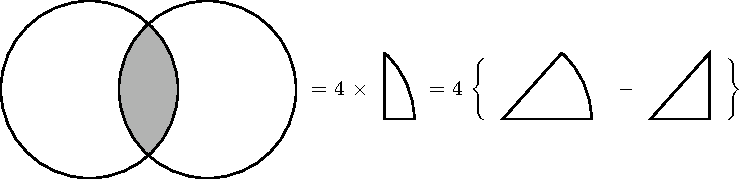
\includegraphics[width = 1.0\textwidth]{../figures/autocorrelation/autocorrelation.pdf}
   \caption{Geometric construction for evaluating the autocorrelation. We need
     to integrate over the overlapping region of two circles with radius $\nu_o$
     and distance $\nu$ between their centers. The region is given by four times
     the difference in area between a sector of angle
     $\arccos\left(\frac{\nu}{2\nu_o}\right)$ and a triangle with base $\nu/2$
     and hypotenuse $\nu_o$.}
   \label{fig:geometry}
 \end{figure}

 We will only evaluate these integrals for $n=1$ and $n=2$, but the result for
 arbitrary $n$ is likely possible as a recurrence relation. For $n=1$:

\begin{align}
  A_1(\nu) &= \frac{4}{\pi\nu_o^{2}}\left[\int_0^{\nu_o}\tau d\tau\int_0^{\cos^{-1}\left(\frac{\nu}{2\nu_o}\right)}d\phi_{\tau} - \int_{0}^{\nu/2}d\tau_x\int_0^{\tau_x\frac{2\nu_o}{\nu}\sqrt{1 - \left(\frac{\nu}{2\nu_o}\right)^2}}d\tau_y\right]\Pi\left(\frac{\nu}{4\nu_o}\right),\\
%  A_1(\nu) &= \frac{4}{\pi\nu_o^{2}}\left[\int_0^{\nu_o}\tau d\tau\cos^{-1}\left(\frac{\nu}{2\nu_o}\right) - \int_{0}^{\nu/2}d\tau_x\tau_x\frac{2\nu_o}{\nu}\sqrt{1 - \left(\frac{\nu}{2\nu_o}\right)^2}\right]\Pi\left(\frac{\nu}{2\nu_o}\right),\\
  A_1(\nu) &= \frac{2}{\pi}\left\{\cos^{-1}\left(\frac{\nu}{2\nu_o}\right) - \frac{\nu}{2\nu_o}\sqrt{1 - \left(\frac{\nu}{2\nu_o}\right)^2}\right\}\Pi\left(\frac{\nu}{2\nu_o}\right).
\end{align}
which is a well-known result \cite{goodman1996, mertz2009}. For $n=2$:
\begin{align}
  A_2(\nu) = \frac{8}{\pi\nu_o^{4}}\Bigg[&\int_0^{\nu_o}\tau d\tau\int_0^{\cos^{-1}\left(\frac{\nu}{2\nu_o}\right)}d\phi_{\tau}(\tau^2 - \nu\tau\cos\phi_{\tau}) - \\ &\int_{0}^{\nu/2}d\tau_x\int_0^{\tau_x\frac{2\nu_o}{\nu}\sqrt{1 - \left(\frac{\nu}{2\nu_o}\right)^2}}d\tau_y\, (\tau_x^2 + \tau_y^2 - \nu\tau_x)\Bigg]\Pi\left(\frac{\nu}{2\nu_o}\right),\\
  A_2(\nu) = \frac{2}{\pi}\Bigg\{&\cos^{-1}\left(\frac{\nu}{2\nu_o}\right) - \left[3 - 2\left(\frac{\nu}{2\nu_o}\right)^2\right]\frac{\nu}{2\nu_o}\sqrt{1 - \left(\frac{\nu}{2\nu_o}\right)^2}\Bigg\}\Pi\left(\frac{\nu}{4\nu_o}\right). 
\end{align}

\section{Spherical Fourier transform of a double cone}\label{sec:cone}
In this appendix we will evaluate the spherical Fourier transform of a
normalized double-cone angular distribution with central direction $\mh{s}'$ and
cone half-angle $\Delta$
\begin{align}
  f_{\text{(cone)}}(\mh{s}; \mh{s}', \Delta) = \frac{1}{2\pi(1 - \cos\Delta)}\Pi\left(\frac{\mh{s}\cdot\mh{s}'}{\cos\Delta}\right). 
\end{align}
The spherical Fourier transform is given by
\begin{align}
  F_{\ell\text{(cone)}}^m(\mh{s}', \Delta) = \int_{\mbb{S}^2}d\mh{s}\, f_{\text{(cone)}}(\mh{s}; \mh{s}', \Delta)\bar{Y}_\ell^m(\mh{s}).
\end{align}
The limits of integration will be difficult to find unless we change coordinates
to exploit the axis of symmetry $\mh{s}'$. Since the spherical function is
rotationally symmetric about $\mh{s}'$ we can rotate the function so that the axis of
symmetry is aligned with $\mh{z}$ and multiply by $\sqrt{\frac{4\pi}{2l+1}}Y_\ell^m(\mh{s}')$ to account for the rotation
\begin{align}
    F_{\ell\text{(cone)}}^m(\mh{s}', \Delta) = \sqrt{\frac{4\pi}{2l+1}}Y_\ell^m(\mh{s}')\int_{\mbb{S}^2}d\mh{s}\, f_{\text{(cone)}}(\vartheta; \mh{z}, \Delta)Y_\ell^0(\mh{s}). 
\end{align}
In this coordinate system the double cone is independent of the azimuthal angle,
so we can evaluate the azimuthal integral and express the function in terms of an
integral over
$\vartheta$
\begin{align}
    F_{\ell\text{(cone)}}^m(\mh{s}', \Delta) = 2\pi Y_\ell^m(\mh{s}')\int_{0}^\pi d\vartheta\, \sin\vartheta f_{\text{(cone)}}(\vartheta; \mh{z}, \Delta)P_\ell(\cos\vartheta). 
\end{align}
The function $f_{\text{(cone)}}(\vartheta; \mh{z}, \Delta)$ is only non-zero on
the intervals $\vartheta \in [0, \Delta]$ and
$\vartheta \in [\pi - \Delta, \pi]$ so
\begin{align}
    F_{\ell\text{(cone)}}^m(\mh{s}', \Delta) = \frac{Y_\ell^m(\mh{s}')}{2(1 - \cos\Delta)}\left[\int_{0}^\Delta d\vartheta\, \sin\vartheta P_\ell(\cos\vartheta) + \int_{\pi - \Delta}^\pi d\vartheta\, \sin\vartheta P_\ell(\cos\vartheta)\right]. 
\end{align}
Applying a change of coordinates with $u = \cos\vartheta$ yields
\begin{align}
    F_{\ell\text{(cone)}}^m(\mh{s}', \Delta) = \frac{Y_\ell^m(\mh{s}')}{2(1 - \cos\Delta)}\left[\int_{\cos\Delta}^1 d\vartheta\, P_\ell(u) + \int_{-1}^{-\cos\Delta} d\vartheta\, P_\ell(u)\right]. 
\end{align}
The Legendre polynomials $P_\ell(u)$ are even (odd) on the interval [-1, 1] when
$\ell$ is even (odd), so the pair of integrals will be identical when $\ell$ is
even and cancel when $\ell$ is odd. For even $\ell$
\begin{align}
  F_{\ell\text{(cone)}}^m(\mh{s}', \Delta) = \frac{Y_\ell^m(\mh{s}')}{1 - \cos\Delta}\int_{\cos\Delta}^1 d\vartheta\, P_\ell(u).
\end{align}
The integral evaluates to \cite{gradshteyn2007} 7.111 
\begin{align}
  \int_{\cos\Delta}^1 d\vartheta\, P_\ell(u) =
\begin{cases}
  1 - \cos\Delta\,, &\ell = 0\,,\\
  \sin\Delta\, P_l^{-1}(\cos\Delta)\,, &\text{else},
\end{cases}
\end{align}
where $P_l^{-1}(\cos\Delta)$ is the associated Legendre polynomial with order
$m=-1$, not an inverse Legendre polynomial. Bringing everything together

\begin{align}
  F_{\ell\text{(cone)}}^m(\mh{s}', \Delta) =
  \begin{cases}
    1, & \ell = 0,\\
    0, & \ell\, \text{odd},\\
    Y_\ell^m(\mh{s}')\cot\left(\frac{\Delta}{2}\right)P_l^{-1}(\cos\Delta), & \ell > 0\,\, \text{even}.
  \end{cases}
\end{align}

\end{document}
